\documentclass{article}

\usepackage{amsfonts}
\usepackage{amsthm}
\usepackage{amsmath}
\usepackage{amssymb}
\usepackage{upgreek}
\usepackage[cm]{fullpage}
%%\usepackage{algorithmic}
%%\usepackage{algorithm} % must read after hyperref
\usepackage[colorlinks={true}, citecolor=blue, linkcolor=blue]{hyperref}       % hyperlinks
\usepackage{algpseudocode}
\usepackage{bbm}
\usepackage{bm}
\usepackage{graphicx}
\graphicspath{{./img/}}
\newtheorem{proposition}{Proposition}

%% \usepackage{array}
%% \usepackage{comment,array,wasysym}
%% \usepackage{graphicx,color,colortbl}

%% % \usepackage{mathptmx} % Use Times as default text font, and provide maths support.  I hate what it does to mathcal so I comment it out
%% % \usepackage{mathtools}
%% % \usepackage{multimedia}
%% % \usepackage{subfigure}
%% %\usepackage{ulem} % for strikethrough \sout
%% \usepackage[normalem]{ulem} % for strikethrough \sout, but avoid the annoying underline in \emph



%% % 
%% % \usepackage[utf8x]{inputenc}
%% % \usepackage{default}

%% % AISTATS sty file doesn't play nicely with caption and subcaption pkgs
%% % \usepackage{caption} 
%% %\usepackage{subcaption}

%% \usepackage{caption}
%% \DeclareCaptionType{copyrightbox}  % Without this, the AISTATs sty creates some clash
%% \usepackage{subcaption}


%% \usepackage{ifthen}
%% \usepackage{enumerate}


%% % 
%% % 
%% %         
%% % \usepackage{yhmath}  % I want really wide tilde. Oren Freifeld, 05/19/2013       




%% %% ICML PACKAGES %%
%% %% \usepackage{ellipsis}

%% %% \usepackage{multirow}

%% %% % Recommended, but optional, packages for figures and better typesetting:
%% %% \usepackage{microtype}
%% %% \usepackage{graphicx}
%% %% % \usepackage{subfigure}
%% %% \usepackage{booktabs} % for professional tables

%% %% % hyperref makes hyperlinks in the resulting PDF.
%% %% % If your build breaks (sometimes temporarily if a hyperlink spans a page)
%% %% % please comment out the following usepackage line and replace
%% %% % \usepackage{icml2018} with \usepackage[nohyperref]{icml2018} above.
%% %% \usepackage{hyperref}

%% %% % Attempt to make hyperref and algorithmic work together better:
%% %% \newcommand{\theHalgorithm}{\arabic{algorithm}}


%% %
%% % Commenting macros
%% %
%% \newcommand{\BLUE}[1]{{{\color{blue}{#1}}}}      
\newcommand{\RED}[1]{{{\color{red}{#1}}}}     
%% \newcommand{\MAGENTA}[1]{{{\color{magenta}{#1}}}}     
%% \definecolor{darkgreen}{rgb}{0,.5,0 }
%% \newcommand{\DARKGREEN}[1]{{{\color{darkgreen}{#1}}}}      
%% \newcommand{\TBD}{\RED{[--TBD--]}}
%% \newcommand{\TODO}[1]{\RED{[--TODO: #1--]}}
%% \newcommand{\BRAINDUMP}[1]{\DARKGREEN{[BRAIN DUMP: #1]}}
%  
%  \newcommand{\OREN}[1]{\RED{[Oren says: #1]}}
% % PICK YOUR COLOR...
\newcommand{\jwf}[1]{\BLUE{<\textbf{JWF}: #1 >}}
% \newcommand{\SUE}[1]{\MAGENTA{[Sue says: #1]}}

% MRF
\newcommand{\pot}{\psi}
\newcommand{\epmarg}{q}
\newcommand{\logpart}{\Phi}

% min / max
\DeclareMathOperator*{\argmax}{arg\,max\;}
\DeclareMathOperator*{\argmin}{arg\,min\;}

% Info Theory Stuff
\newcommand{\KL}[2]{\mathrm{KL}(#1\,\|\,#2)}

%
% List macros
%
\newcommand{\bi}{\begin{itemize}}
\newcommand{\ei}{\end{itemize}}
\newcommand{\deriv}{\mathrm{d}}

\newcommand{\etal}{\textit{et al}}
\newcommand{\FIG}{Fig.~}
%\newcommand{\FIGS}{Figs.~}

 \newcommand{\SEC}{Sec.~}

\newcommand{\eg}{\textit{e.g.}~}
\newcommand{\ie}{\textit{i.e.}~}
\newcommand{\cf}{\textit{c.f.}~}


\newcommand{\EQN}{Eqn.~}
% \newcommand{\EQN}{Equation }
\newcommand{\EQNS}{Eqns.~}
% \newcommand{\EQNS}{Equations }

% Expectation and Probability
\newcommand{\EE}{\ensuremath{\mathbb{E}}}
\newcommand{\PP}{\ensuremath{\mathbb{P}}}


% distributions
\newcommand{\Dir}{\ensuremath{\text{Dirichlet}}}
 
% integers
\newcommand{\ZZ}{\ensuremath{\mathbb{Z}}}
\newcommand{\RR}{\ensuremath{\mathbb{R}}}
\newcommand{\Rtwo}{\ensuremath{\RR^2}}
\newcommand{\Rthree}{\ensuremath{\RR^3}}
\newcommand{\Rn}{\ensuremath{\RR^n}}
% 
%positive integers
\newcommand{\Zplus}{\ensuremath{\ZZ^+}}
%positive reals
\newcommand{\Rplus}{\ensuremath{\RR^+}}


% n by n matrices
\newcommand{\nBynMats}{\ensuremath{\RR^{n \times n}}}
% m by n matrices
\newcommand{\mBynMats}{\ensuremath{\RR^{m \times n}}}
% n by p matrices
\newcommand{\nBypMats}{\ensuremath{\RR^{n \times p}}}
% 2 by 2
\newcommand{\TwoByTwoMats}{\ensuremath{\RR^{2 \times 2}}}
% 3 by 3
\newcommand{\ThreeByThreeMats}{\ensuremath{\RR^{3 \times 3}}}
% 2 by 3
\newcommand{\TwoByThreeMats}{\ensuremath{\RR^{2 \times 3}}}




% \newcommand{\EqualsDef}{\,{\overset{\text{def}}{=}}\,}
\newcommand{\EqualsDef}{\triangleq}


% set notation
% \newcommand{\set}[1]{\ensuremath{{\left\{#1\right\}}}}
\newcommand{\set}[1]{\ensuremath{{\{#1\}}}}


\newcommand{\InnerProduct}[2]{\left\langle #1,#2 \right\rangle}

\newcommand{\norm}[1]{{{\left\|#1\right\|}}}
\newcommand{\sign}[1]{{\mathrm{sign}\left(#1\right)}}


\newcommand{\ellTwoNorm}[1]{\norm{#1}_{\ellTwo}}


\newcommand{\Acal}{\mathcal{A}}
\newcommand{\Bcal}{\mathcal{B}}
\newcommand{\Ccal}{\mathcal{C}}
\newcommand{\Dcal}{\mathcal{D}}
\newcommand{\Ecal}{\mathcal{E}}
\newcommand{\Fcal}{\mathcal{F}}
\newcommand{\Gcal}{\mathcal{G}}
\newcommand{\Mcal}{\mathcal{M}}
\newcommand{\Ncal}{\mathcal{N}}
\newcommand{\Ocal}{\mathcal{O}}
\newcommand{\Pcal}{\mathcal{P}}
\newcommand{\Qcal}{\mathcal{Q}}
\newcommand{\Tcal}{\mathcal{T}}
\newcommand{\Vcal}{\mathcal{V}}
\newcommand{\Wcal}{\mathcal{W}}
\newcommand{\Xcal}{\mathcal{X}}
\newcommand{\Ycal}{\mathcal{Y}}

\newcommand{\MATRIX}[2][cccccccccccccccccccc]{\left[
 \begin{array}{#1}
 #2
 \end{array}
\right]}


\newcommand{\TRACE}{\mathrm{trace}}

\newcommand{\var}[1]{\text{var} \big( #1 \big) }
\newcommand{\cov}[2]{\text{cov} \big( #1,#2 \big)}
\newcommand{\myt}[1]{\widetilde {#1} }

% bold font math 
\bmdefine\balpha{\alpha}
\bmdefine\bbeta{\beta}

\bmdefine\bphi{\phi}


\bmdefine\bb{b}

\bmdefine\bx{x}
\bmdefine\by{y}
\bmdefine\bdotx{\dot{x}}
\bmdefine\bxzero{x_{0}}
\bmdefine\bxone{x_{1}}

\bmdefine\bu{u}

\bmdefine\bv{v}
\bmdefine\br{r}


\bmdefine\bA{A}
\bmdefine\bB{B}

\bmdefine\bS{S}

\bmdefine\bU{U}

\bmdefine\bV{V}
\bmdefine\bX{X}
\bmdefine\bY{Y}


%\bmdefine\balpha{\alpha}

 \newcommand{\Nc}{{N_{c}}}
% \newcommand{\Nc}{N}
\newcommand{\Ne}{{N_{e}}}

% homo coo
\newcommand{\bxh}{\widetilde{\bx}}




\newcommand{\GLn}{\ensuremath{\mathrm{GL(n)}}}
\newcommand{\gln}{\ensuremath{\mathfrak{gl(n)}}}

\newcommand{\GLone}{\ensuremath{\mathrm{GL(1)}}}
\newcommand{\GLtwo}{\ensuremath{\mathrm{GL(2)}}}
\newcommand{\glTwo}{\ensuremath{\mathfrak{gl}(2)}}


% CPA Stuff

\newcommand{\Ac}[1]{A_{c(#1)}}
\newcommand{\Bc}[1]{B_{c(#1)}}

\newcommand{\Vaff}{\Vcal_{\mathrm{aff}}}

\newcommand{\Vpa}{\Vcal_{\mathrm{PA}}}
\newcommand{\Vcpa}{\Vcal_{\mathrm{CPA}}}


\newcommand{\Faff}{\Fcal_{\mathrm{aff}}}

\newcommand{\Fpa}{\Fcal_{\mathrm{PA}}}
\newcommand{\Fcpa}{\Fcal_{\mathrm{CPA}}}

\newcommand{\NSTEPS}{N_{\mathrm{STEPS}}}
\newcommand{\nsteps}{n_{\mathrm{steps}}}


\newcommand{\SigmaPA}{\Sigma_{\mathrm{PA}}}

\newcommand{\SigmaCPA}{\Sigma_{\mathrm{CPA}}}



\newcommand{\Vat}[1]{\bv{(#1)}}
\newcommand{\VatX}{\Vat{\bx}}
\newcommand{\Tat}[2]{T{(#1,#2)}}
\newcommand{\Tinvat}[2]{T^{-1}{(#1,#2)}}
\newcommand{\VatT}[1][t]{\Vat{\Tat{\bx}{#1}}}
% \newcommand{\VatT}[1][t]{\Vat{\Tat{\bx,#1}}}
\newcommand{\VatTinv}[1][t]{\Vat{\Tinvat{\bx}{#1}}}


\newcommand{\IntVatTofX}[1][t]{\int_{0}^{#1}\VatT[\tau]\, d\tau}

\newcommand{\AtimesX}{A{\bxh}}
 

\newcommand{\CpaVatX}{\Ac{\bx}\bxh}
% \newcommand{\CpaVatT}[1][t]{\Ac{\Tat{\bx}{#1}}\widetilde{T}(\bx,#1)}
\newcommand{\CpaVatT}[1][t]{\Ac{\Tat{\bx}{#1}}\widetilde{\Tat{\bx}{#1}}}

\newcommand{\IntCpaVatT}[1][t]{\int_{0}^{#1} \CpaVatT[\tau] \, d\tau}


 

\newcommand{\IntCpaVatTinv}[1][t]{\int_{0}^{#1}  \Ac{\Tinvat{\by}{#1}}\widetilde{\Tinvat{\by}{#1}} \, d\tau}


\newcommand{\CpaVatXasLinComb}{\sum_{j=1}^{d}\alpha_k\Bc{\bx}^{j}\bxh}
\newcommand{\CpaVatTasLinComb}[1][t]{\sum_{j}^{d}\alpha_j\Bc{\Tat{\bx}{#1}}^{j}\widetilde{\Tat{\bx}{#1}}}


\newcommand{\IntCpaVatTLinComb}[1][t]{\int_{0}^{#1}  \CpaVatTasLinComb[\tau] \, d\tau}


% USAGE:
% $\Vat{\bx}$
% $\VatX$
% $\Tat{\bx}{t}$
% $\VatT$
% $\VatT[\tau]$
% $\VatTinv[\tau]$
% $\IntVatTofX$
% $\AtimesX$
% $\Ac{\bx}$
% $\CpaVatX$
% $\IntCpaVatT$
% $\CpaVatXasLinComb$
% $\IntCpaVatTLinComb$



%\newcommand{\VEE}[1]{{#1}^{\vee}}
\newcommand{\VEE}[1]{\mathrm{vec}({#1})}

\newcommand{\HAT}[1]{{#1}^{\wedge}}

 \newcommand{\LCONSTRAINTS}{L_{\mathrm{constraints}}}

% Graph stuff
\newcommand{\parent}{\text{Pa}}
\newcommand{\interventions}{\mathcal{I}}
\newcommand{\alldata}{\mathcal{X}}

% Planning stuff
\newcommand{\actionset}{\mathcal{A}}



%% DOCUMENT %%%%%%%%%%%%%%%%%%%%%%%%%%%%%%
\begin{document}

%% TITLE %%%%%%%%%%%%%%%%%%%%%%%%%%%%%%%%%
\title{Variational Information Planning Notes}
\author{Jason Pacheco}
\maketitle

\section{Information Theoretic Planning}

Consider a model of latent variables $x$ and conditionally
independent observations $\Ycal_T = \{y_1,\ldots,y_T\}$.  At each time
$t$ a discrete \emph{action} $a_t \in \{1,\ldots,A\}$ parameterizes
the likelihood, denoted \mbox{$p_{a_t}(y_t \mid x)$}.  Given
observations $\Ycal_T$ and actions $\actionset_T = \{a_1,\ldots,a_T\}$
the posterior is:
\begin{equation}\label{eq:joint}
  p(x\mid \Ycal_T; \actionset_T) \propto p(x) \prod_{t=1}^T p_{a_t}(y_t \mid x)
\end{equation}
The choice of conditionally independent observations in the joint is
for simplification.  Our approach is easily extended to the case where
nuisance variables must be integrated out, as shown in the labeled LDA
example of Sec.~\ref{sec:llda}.  Given the posterior at stage $t-1$
information thoretic planning selects an action to maximize the
posterior mutual information (MI):
%% Using uppercase letters $Y$
%% to denote a random variables and lowercase $y$ to denote their
%% realization, we have the posterior MI:
%% \begin{align}\label{eq:mi_integral}
%% a_t^{*} &= \argmax{a_t\in\actionset} \;I(X; Y_t | \Ycal_{t-1}; a_t ) \\  
%%   &=  \int p_{a_t}( x, y_t  |  \Ycal_{t-1} ) \log \frac{p_{a_t}(y_t | x)  }
%%     {p_{a_t}( y_t | \Ycal_{t-1} )} \deriv x \deriv y_t. \notag
%% \end{align}
\begin{align}\label{eq:mi_integral}
  a_t^{*} &= \argmax{a} \;I_a(X; Y_t \mid \Ycal_{t-1} ) \\
  &= \argmax{a} \;H(X \mid \Ycal_{t-1} ) - H_a(X \mid Y_t, \Ycal_{t-1}) \notag
\end{align}
where $H_a( \cdot )$ denotes differential entropy under the
hypothesized action $a$.  Under this model the marginal entropy
$H(X\mid \Ycal)$ summarizes past observations and is thus invariant to
the choice of action at time $t$.  Having chosen action $a^{*}_t$ the
system draws a new observation from the corresponding likelihood: $y_t
\sim p_{a^{*}_t}(\cdot \mid x)$.  The posterior is then updated and
the process is repeated.  Note that this procedure can be interpreted
as a general case of Bayesian sequential experiment design.


\section{Variational Information Planning}

Calculation of MI~\eqref{eq:mi_integral} is complicated by the
posterior expectations required to calculate entropy.  In this section
we show a variational lower bound on MI that is maximized through
moment-matching.  We conclude with a brief description of a fully
variational inference and planning algorithm.

\subsection{Variational Information Bound}

For any valid distribution $q\in\Qcal$ we have the following lower
bound:
\begin{equation}\label{eq:varmi}
  I(X;Y_t \mid \Ycal_{t-1} ) \geq H(X \mid \Ycal_{t-1}) - H_p( q(X\mid
  Y_t) ) 
  % &= H(X \mid \Ycal_{t-1}) + \big\langle\, \log q(X \mid Y_t) \,\big\rangle_{p(x,y_t \mid
  %   \Ycal_{t-1})}
\end{equation}
where the final term is the cross-entropy: $H_p(q(x\mid y)) =\langle -
\log q(x\mid y) \rangle_{p(x,y)}$.  The bound is a result of the
nonnegativity of Kullback-Leibler divergence since $KL(p\|q) \geq 0$,
then $H(p) \geq H_p(q)$ and is tight when $q(X \mid Y_t)$ equals the
posterior $p(X \mid Y_t, \Ycal_{t-1})$.  When $q\in\Qcal$ is an
exponential family distribution the tightest bound is achieved via
moment-matching.  To see this we rewrite bound~\eqref{eq:varmi} as an
equivalent constrained maximization over natural parameters:
\begin{equation}\label{eq:constrained_varmi}
  \max_q H(x) + H_p( q(y) ) - H_p(
  q(x,y) ) \;\;\;\text{such that}\;\;\; q(y) = \int q(x,y) dx
\end{equation}
For brevity we have dropped explicit conditioning on the observation
set $\Ycal$ and time index subscripts $t$.  The marginalization
constraint ensures $q(x \mid y)$ is a valid conditional distribution.
Rearranging the objective we have the equivalent minimization:
\begin{equation}\label{eq:moment_match}
  q^{*} = \argmin{q(x,y)} \KL( p(x,y) \| q(x,y) ) - \argmin{q(y)} \KL(p(y) \| q(y))
\end{equation}
The above minimization is \emph{equivalent} in the sense that $q^{*}$
is the maximizer of~\eqref{eq:constrained_varmi} and the minimizer
of~\eqref{eq:moment_match}, though their objective functions differ.
However, the moment-matching property of exponential families ensures
that~\eqref{eq:moment_match} is a convex objective whose unique
solution corresponds to matching the expected sufficient statistics of
$q$ to the corresponding moments of $p$.  We choose $q(x,y)$ so that
$q(y) = \int q(x,y) dx$ remains in the exponential family.  This
choice of $q(x,y)$ ensures that the solution to the unconstrained
objective satisfies the marginalization constraints.


%% \begin{align}
%%   q(x,y) &= \exp\{ \eta^T \phi(x,y) - A(\eta) \} \\
%%   q(y) &= \exp\{ \lambda^T \phi(y) - A(\lambda) \}
%% \end{align}


\subsection{Algorithm Description}

Suppose that at time $t-1$ we have a posterior approximation $q(x)
\approx p(x \mid \Ycal_{t-1})$.  For each hypothesized action $a_t \in
\Acal$ we construct a local approximation of the joint distribution.
The local approximation consists of the variational posterior, which
summarizes previous observations, and the predicted future observation
conditioned on the hypothesized action:
\begin{equation}
  \hat{p}_{a_t}(x,y_t \mid \Ycal_{t-1}) \propto q(x) p_{a_t}(y_t \mid x)
\end{equation}
Our variational planning
objective maximizes the lower bound~\eqref{eq:varmi} of MI under the
approximation $\hat{p}$,
\begin{equation}
  \max_{a\in\Acal} I_{\hat{p}_a}(X;Y_t \mid \Ycal_{t-1} ) \geq
  \max_{a\in\Acal} \max_{q_a\in\Qcal} H_{\hat{p}}(X \mid \Ycal_{t-1}) - H_{\hat{p}_a}(
  q_a(X\mid Y_t) ).
\end{equation}
As was shown in the previous section, the lower bound for each action
can be found by matching moments of $q_a$ and $\hat{p}$.  This
procedure of moment-matching to a local approximation is analogous to
the steps in expectation propagation (EP).  More specifically, the
local approximation $\hat{p}$ is analogous to the \emph{augmented
  distribution} in EP.  The model requirement is that expected
sufficient statistics under $\hat{p}$ can be calculated efficiently.
Planning requires a total of $\Ocal( |\Acal| )$ moment-matching
operations, which can be done in parallel.



\section{Labeled LDA Example}\label{sec:llda}

\begin{figure}[t]
  \centering
  \begin{tabular}{ccc}
    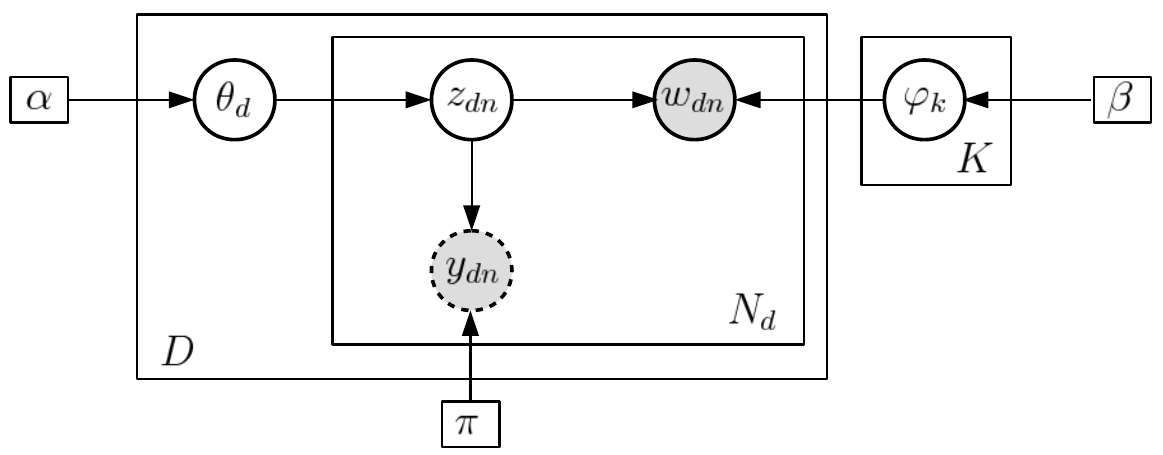
\includegraphics[height=0.14\textheight]{llda_model.png} &
    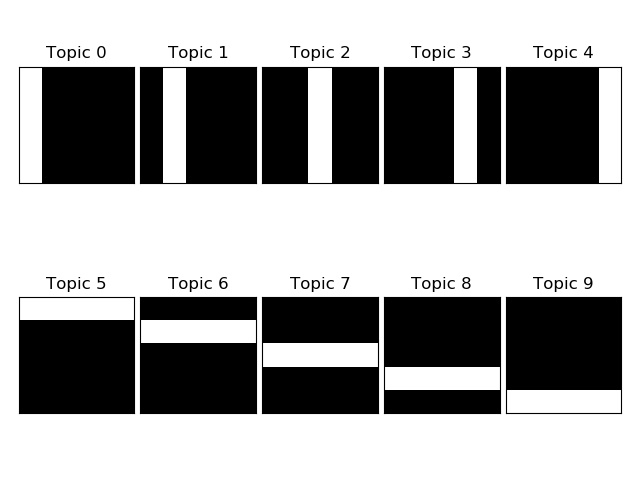
\includegraphics[height=0.14\textheight]{BARS_10.png} &
    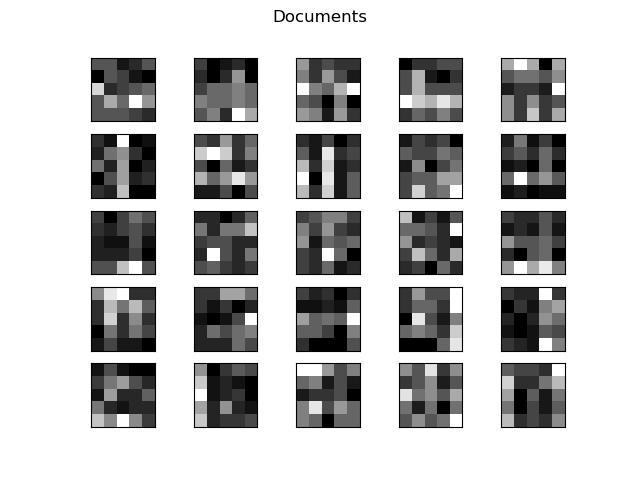
\includegraphics[height=0.14\textheight]{BARS_docs.png} \\
    {\small \textbf{Model}} & {\small \textbf{``Bars'' Topics}} & {\small \textbf{Sample Documents}}
  \end{tabular}
  \caption{\small \textbf{Labeled LDA} The graphical model of LLDA
    denotes semi-supervised annotation $y_{dn}$ with a dashed line.
    Each word $n$ of document $d$ is assigned an annotation and at
    each planning stage we select among the remaining set of
    annotations.  We use synthetic ``bars'' topics as introduced in
    Griffiths and Steyvers.}
  \label{fig:llda}
\end{figure}

Labeled LDA (LLDA), introduced in Flaherty et al. (2005), extends LDA
to include a semi-supervised label for each word in the corpus.  The
application considered in Flaherty et al. uses LLDA to infer latent
groups of genes affected by various drugs.  In that setting the
annotation label assigns functional categories to individual genes,
when they are known.  In this way the LLDA model can discover
interpretable topics.  See Fig.~\ref{fig:llda} for the LLDA graphical
model and notation we will reference below.

At stage $t-1$ of learning we observe a set of annotations
$\Ycal_{t-1} = \{ y_{d_1 n_1}, \ldots, y_{d_{t-1} n_{t-1}}\}$, which
we treat as discrete in this example.  We update our variational
posterior approximation over $K$ topics $\varphi$ and document-topic
proportions $\theta$ for $D$ documents:
\begin{equation}
  p(\theta, \varphi \mid \Ycal_{t-1}) \approx \prod_{d=1}^D q(\theta_d)
  \prod_{k=1}^K q(\varphi_k)
\end{equation}
During stage $t$ \emph{planning} we select the index $(d,n)$ which
maximizes MI between topics $\varphi$ and annotation $Y_{dn}$ as in:
$\max_{d,n} I(Y_{dn}; \varphi \mid \Ycal_{t-1})$.  Unlike the simplef
model~\eqref{eq:joint}, LLDA involves nuisance variables which must be
marginalized during the planning stage.  To generalize the algorithm
we assume an EP-style variational approximation which are product
distributions consisting of \emph{messages} from each neighbor:
\begin{equation}
  q(\varphi_k) = \Dir( \varphi_k \mid \beta + \sum_{d=1}^D
  \sum_{n=1}^N \chi_{kdn} ), \qquad
  q(\theta_d) = \Dir( \theta_d \mid \alpha + \sum_{n=1}^N \upxi_{dn} )
\end{equation}
To form a local approximation we first remove the influence of the
$(d,n)^{th}$ component by subtracting the corresponding natural statistic:
\begin{equation}
   q_k^{\backslash dn}(\varphi_k) = \Dir( \varphi_k \mid \beta +
   \sum_{d=1}^D \sum_{n' \neq n} \chi_{kdn'} ), \qquad
   q_d^{\backslash n}(\theta_d) = \Dir( \theta_d \mid \alpha + \sum_{n' \neq n}
   \upxi_{dn'} )
\end{equation}
The factor $q_k^{\backslash dn}(\varphi_k)$ represents the
distribution on topic $\varphi_k$ after removing influence of word $n$
in document $d$.  Similarly, $q_d^{\backslash n}(\theta_d)$ is the
residual distribution on document-topic proportions.  In EP these are
sometimes referred to as the \emph{cavity} distributions.  The local
approximation is thus a Dirichlet-Multinomial mixture:
\begin{align}
  \hat{p}(\varphi, y_{dn} \mid \Ycal_{t-1}) &\propto \left[ \prod_k
        q_k^{\backslash dn}(\varphi_k) \right] \sum_k \pi_k(y_{dn})
        \varphi_k(w_{dn}) \EE_{q_d^{\backslash n}} \left[ \theta_d(k)
      \right] \\
  &\propto \sum_k C_k \pi_k(y_{dn}) \Dir( \varphi_k \mid \cdot )
\end{align}
Mixture weights $C_k$ and Dirichlet parameters can be easily
calculated, though we omit the details for brevity.  For planning we
approximate $\hat{p}$ with a single Dirichlet-Multinomial distribution
via moment-matching.  We can thus easily calculate the variational
bound on MI used in planning.

\begin{figure}[t]
  \centering
  \begin{tabular}{cc}
    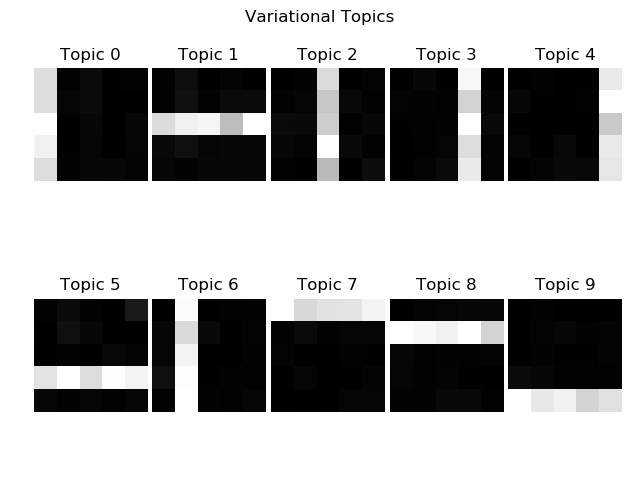
\includegraphics[width=0.45\textwidth]{vartop} &
    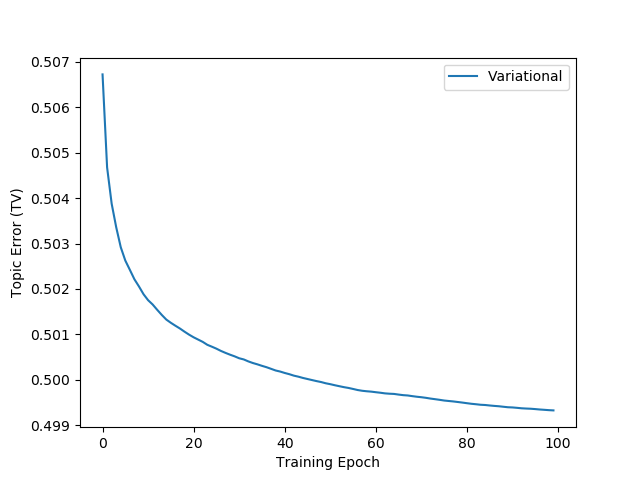
\includegraphics[width=0.45\textwidth]{tv.png}
  \end{tabular}
  \caption{\small \textbf{Preliminary Results} \emph{Left:} Posterior
    mean of inferred topics.  \emph{Right:} Total variation error of
    estimated topics.  The posterior distribution concentrates on the
    correct topic ordering in the limit as all annotations are
    provided.  As a result, the TV error thus penalizes incorrect
    orderings.}
  \label{fig:llda_results}
\end{figure}

As a preliminary experiment we fit LLDA to a simulated dataset of
$D=500$ documents, each with $N=100$ words, and we use the \emph{bars}
dataset introduced in Griffiths and Steyvers.  Specifically, when
topics are arranged into a $5\times 5$ square they place equal
probability in a single column or row, and zero probability elsewhere.
The annotation distribution assigns $y_{dn} = z_{dn}$ with probability
proportional to $1-\epsilon$ and $\epsilon$ otherwise.  In this way
annotations act as true topic assignments with high probability.  We
thus expect topic ordering to stabilize in the limit as all words are
labeled, with the topic posterior concentrating on the correct
ordering.  Fig.~\ref{fig:llda_results} shows results after 100
training rounds.

\end{document}
